Um programa de computador é expresso por um conjunto de sentenças em alguma
linguagem de programação\footnote{Uma sentença (\emph{statement}) pode conter uma ou várias expressões ou instruções.
Uma única instrução numa linguagem de alto nível pode representar múltiplas
instruções de máquinas.
Programas consistem de instruções e expressões.
Uma expressão é um grupo de símbolos que representa um valor.}\todo[fancyline]{Trazer o conteúdo do rodapé pra cá?}.
A forma como as sentenças de uma linguagem são executadas pelo computador é
definida por um \emph{modelo de computação} \cite{vanroy2004}.

O código fonte de um programa consiste de uma série de instruções que expressam
uma sequência de comandos a se seguir durante a execução — esse período é
conhecido como \emph{tempo de execução}, do inglês \emph{runtime}.
Tradicionalmente, as sentenças de uma linguagem de programação denotam essa
sequência de forma explícita.
Tais linguagens são baseadas no modelo \emph{imperativo} de computação, e são
denominadas \emph{linguagens imperativas}.
\section{Linguagens de programação}
\label{sec:linguagens-de-programacao}
\label{sec:langs}

Linguagens de programação são mais simples que linguagens naturais, no
entanto, elas ainda podem conter uma sintaxe surpreendentemente rica, um
conjunto de abstrações, e bibliotecas auxiliares.
Esse é essencialmente o caso de linguagens usadas para resolver problemas
reais do dia-a-dia.
\textcite{vanroy2004} as chamam de linguagens \emph{práticas}, que são “\textelp{}
como a caixa de ferramentas de um mecânico experiente: há várias ferramentas
diferentes para finalidades diferentes e todas estão lá por uma razão.” (p.
33; tradução nossa).

Todas as linguagens de programação possuem elementos primitivos para a
descrição de dados e das transformações, ou processos, aplicados à eles —
como a adição de dois números ou a seleção de um item de uma coleção.
Essas primitivas são definidas por regras de sintaxe — a gramática — e pela
semântica — o significado.

Um programa orientado a eventos reage ao que acontece no ambiente externo: o
clique num botão, a tecla digitada, a mensagem do servidor
\cite[p. 86:1]{madsen2017}.
Os eventos entram numa fila, e o programa os trata um de cada vez
\cite[p. 86:1]{madsen2017}, sem garantia da sequência em que chegam:
como a interação depende de eventos externos, que podem ocorrer em
qualquer ordem, entender o programa exige seguir várias cadeias de causa
e efeito \cite[p. 125]{martin2022}.
A reação depende também do \emph{estado} da aplicação, que determina a
aparência e o comportamento dela \cite[p. 230]{oney2012}.
Uma barra de ferramentas, por exemplo, fica encaixada acima da área de
trabalho até que o usuário a segure pelo topo, gesto que muda o estado
dela: a barra se solta e passa a seguir o mouse \cite[p. 230]{oney2012}.

Nas linguagens imperativas, esse estado é implícito e muda por comandos,
como a atribuição de um valor a uma variável, e essas mudanças são os
\emph{efeitos colaterais} dos comandos \cite[p. 361]{hudak1989}.
Por isso, para controlar o estado com precisão e de forma determinística,
elas costumam fixar a ordem em que os comandos se executam
\cite[p. 361]{hudak1989}.
Numa interface, é o programador quem escreve essa ordem: para cada mudança
de estado, ele precisa escrever a atualização de tudo o que depende do
valor alterado, e esse código é complexo e propenso a erros, como o que
muda o estado na hora errada ou na ordem errada
\cite[p. 52:2]{bainomugisha2013}.
Para \textcite[p. 929]{edwards2009}, boa parte da sequência que o
programador escreve poderia ficar a cargo da execução, ao menos nas
aplicações interativas.

Nas linguagens declarativas, não há estado implícito, e o programa se
escreve com expressões \cite[p. 361]{hudak1989}.
Na \gls{pr}, a ordem das atualizações não se escreve: o ambiente de
execução propaga a mudança de um valor às computações que dependem dele
e as recalcula na ordem do grafo de dependências, cada uma depois das que
ela usa \cite[p. 52:5 e 52:7]{bainomugisha2013}.
A programação declarativa costuma ser descrita como a que expressa “o
quê” e não “o como” da computação, embora a diferença seja de grau
\cite[p. 361]{hudak1989}.
\section{Paradigmas e modelos de programação}
\label{sec:paradigmas-e-modelos-de-programacao}
\todo{Trecho vindo da introdução no corte de outubro de 2026, ainda por integrar a esta seção.}

O modelo de programação não é o paradigma, noção imprecisa que o modelo
de computação torna precisa \cite[p. xiii]{vanroy2004}.
Também não é a biblioteca nem o \emph{framework}, que classificam o produto: o
Web Component, recurso do próprio navegador \cite{mozilla2026}, não é
nenhum dos dois e tem um modelo de programação como as outras
tecnologias.

Cada modelo de programação aplica conceitos de um ou mais paradigmas.
Em quase todo problema, cada parte pede o seu conjunto de conceitos
\cite[p. 10]{vanroy2009}, e as implementações deste trabalho também os
misturam.

As aplicações orientadas a eventos e interativas, na literatura de
\gls{pr}, também se chamam reativas \cite[p. 1125]{salvaneschi2017}, mas
a palavra tem sentidos diferentes em linguagens de programação e em sistemas
distribuídos \cite[5:1]{myter2019} e já nomeia tecnologias como o React
\cite[p. 13]{grolaux2026}.
Por isso, este trabalho as chama de interativas e reserva “reativo” para a
\gls{pr}.

Programação é uma disciplina extensa, e linguagens práticas de programação
geralmente são bastante complicadas.
Felizmente, as ideias importantes de linguagens de programação são simples
\cite{vanroy2009}.
Um \emph{paradigma de programação}:

\begin{citacao}
  \textelp{} é uma abordagem para a programação de um computador baseada em
  uma teoria matemática ou um conjunto coerente de princípios.
  \cite[p.~10; tradução nossa]{vanroy2009}
\end{citacao}

É mais interessante focar em paradigmas de programação do que em linguagens,
porque há muito menos paradigmas que linguagens, como pode-se notar na Figura
\ref{img:LangsParadigmsConcepts} \cite{vanroy2009}.
Segundo \textcite{vanroy2009}:

\begin{citacao}
  Os conceitos são os elementos primitivos básicos usados para construir os
  paradigmas. Muitas vezes dois paradigmas que parecem muitos diferentes (por
  exemplo, programação funcional e programação orientada a objetos) diferem
  por apenas um conceito. (p. 13; tradução nossa)
\end{citacao}

\begin{figure}[ht]
  \caption{Linguagens, paradigmas, e conceitos de programação.} \centering
  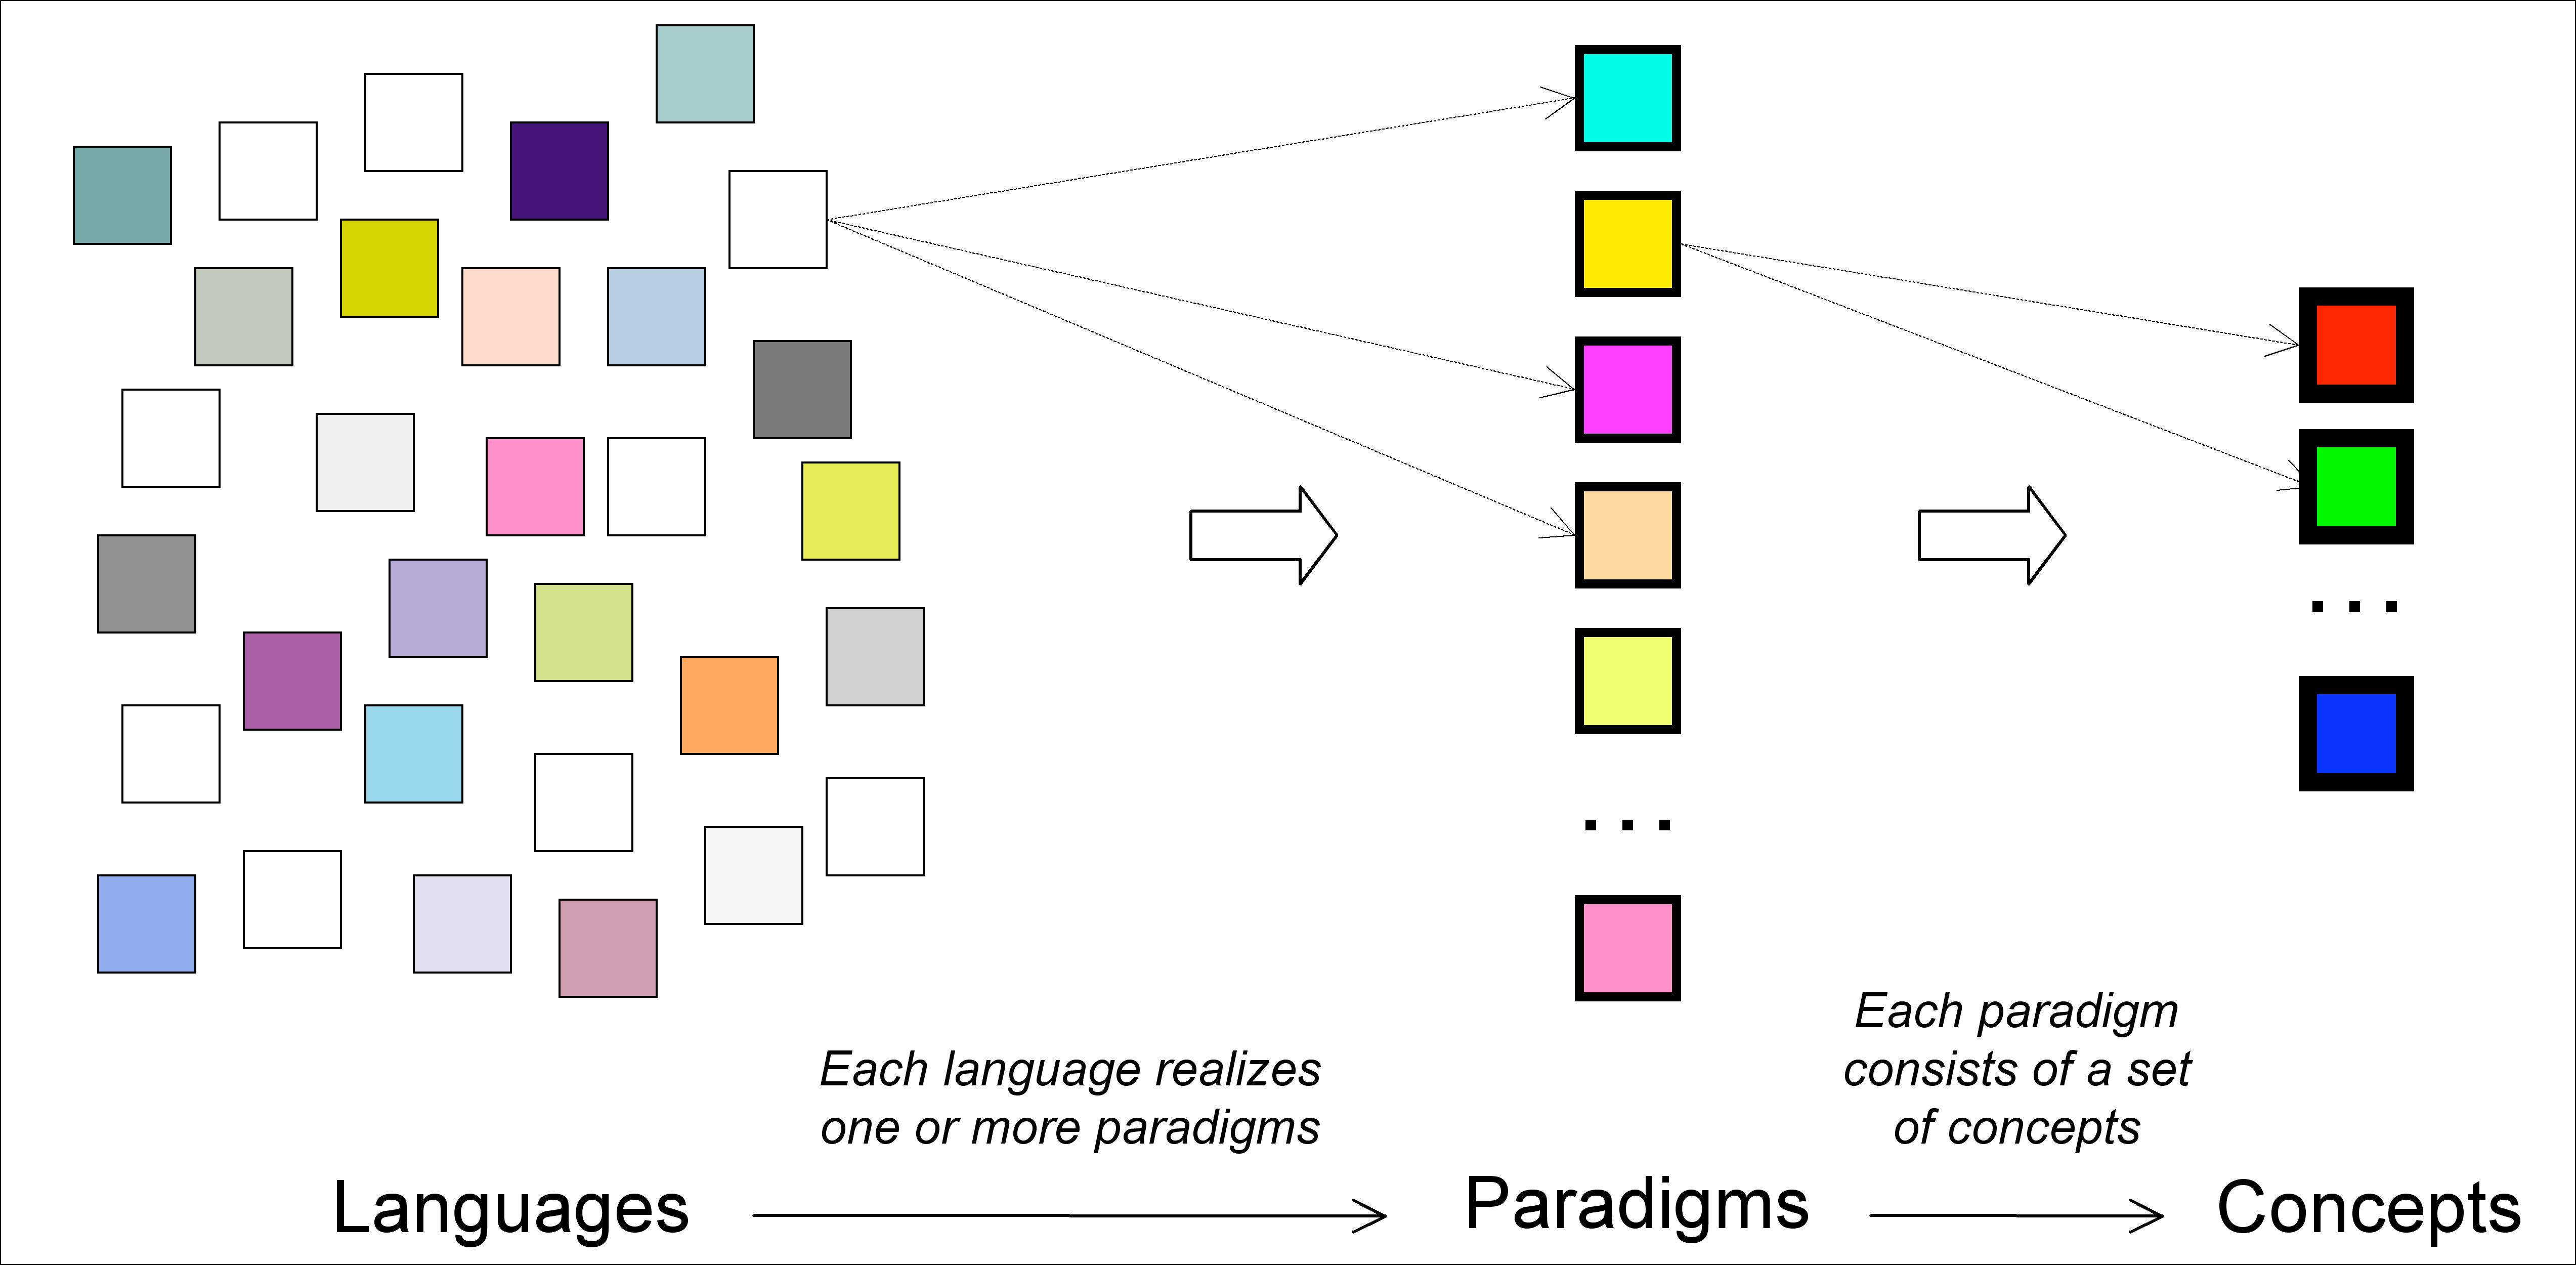
\includegraphics[width=12cm]{./fig/roy2009_languages_paradigms_and_concepts.jpeg}

  \small Fonte: \textcite[p.~12]{vanroy2009}.
  \label{img:LangsParadigmsConcepts}
\end{figure}

Da mesma forma que em engenharia de software (como um processo) pode-se adotar
diferentes metodologias de desenvolvimento, em linguagens de programação (como
modelos de computação) é desejável utilizar diferentes paradigmas de
programação.
Linguagens tradicionais como Java e C++ dão suporte a um ou dois paradigmas
diferentes.
“Isso é lamentável, pois problemas de programação diferentes precisam de
conceitos diferentes de programação para serem resolvidos claramente.”
\cite[p. 10]{vanroy2009}.

\textcite{vanroy2009} defende o uso de um modelo de programação \emph{multiparadigma},
porque:

\begin{citacao}
  Idealmente, uma linguagem deveria dar suporte a vários conceitos de forma
  bem integrada, para que o programador possa escolher os conceitos certos
  sempre que forem necessários, sem que um complique o outro.
  (p.~10; tradução nossa)
\end{citacao}

Apesar de linguagens tradicionais não dar suporte a esse modelo, entender os
conceitos certos pode melhorar a forma de programação, mesmo em linguagens que
não dê suporte direto a eles, assim como programação orientada a objetos é
possível em C com a atitude adequada \cite{vanroy2009}.

\textcite{vanroy2009} apresenta quatro modelos importantes que simplificam
programação concorrente em relação à linguagens convencionais: \emph{concorrência
declarativa}, \emph{programação funcional reativa}, \emph{programação síncrona
discreta}, e \emph{programação com restrições}.

No modelo declarativo de concorrência o resultado de um programa pode ser
calculado incrementalmente.
“Se a entrada de um programa concorrente é dada incrementalmente, então o
programa também irá calcular o resultado de saída incrementalmente.”
\cite[p. 238; tradução nossa]{vanroy2004}.
Esses paradigmas não possuem condições de corrida, \emph{‘race conditions’} em
inglês.
\todo{Esses últimos dois parágrafos parecem estar deslocados.}
\section{Programação de interfaces gráficas}
\label{sec:programacao-de-interfaces-graficas}
\todo{Trecho vindo da introdução no corte de outubro de 2026, ainda por integrar a esta seção.}

No projeto da interface, além dos problemas comuns a todo sistema de
software complexo, os \emph{designers} lidam com tarefas e domínios complexos e
têm dificuldade de pensar como o usuário \cite[p. 75]{myers1994}.
Na implementação, o programa também precisa ser robusto: tratar qualquer
entrada sem parar de funcionar e, como o usuário espera, permitir que ele
cancele e desfaça a maioria das ações \cite[p. 75, 79 e 80]{myers1994}.

O \emph{callback} é síncrono quando a função que o recebe o chama antes de
retornar, e assíncrono quando sua execução fica para algum tempo depois de a
função retornar \cite[p. 2]{gallaba2015}.
O navegador executa a aplicação numa \emph{thread} só, e, para que ela continue
respondendo ao usuário, os programadores recorrem às operações assíncronas
\cite[p. 368-369]{alimadadi2014}.
O \emph{callback} de um clique é desse tipo: registrado quando a tela é montada,
só roda quando o usuário clica, e os eventos do \gls{dom} estão entre as
operações assíncronas do navegador \cite[p. 5]{gallaba2015}.

\emph{Threads} exprimem sequência, e eventos exprimem dependência, e muitos
problemas vêm de escrever uma com o recurso da outra
\cite[p. 16]{blackheath2016}.

Em JavaScript, os \emph{callbacks} são frequentes: num estudo de 138 programas, em
média uma em cada dez definições de função recebe um \emph{callback}, e a maioria dos
\emph{callbacks} é aninhada \cite[p. 1]{gallaba2015}.
No código do navegador, em média 9\% das chamadas de função passam um
\emph{callback}, e 72\% desses \emph{callbacks} são assíncronos \cite[p. 6]{gallaba2015}.
Numa sessão típica de uso de onze sites, como Gmail, Facebook e Amazon, os
tratadores de eventos executam de 31,6\% a 99,1\% das instruções JavaScript
\cite{ratanaworabhan2010}.

O JavaScript ganhou alternativas ao \emph{callback}: as \emph{promises}, que encadeiam
computações assíncronas \cite[p. 86:1]{madsen2017}, e as palavras-chave
\emph{async} e \emph{await}, que permitem escrever operações assíncronas em estilo
sequencial \cite[p. 9]{grolaux2026}.
As \emph{promises} achatam o aninhamento dos \emph{callbacks}, mas a lógica complexa
continua presa em cadeias de \emph{callbacks} \cite[p. 9]{grolaux2026}.
Numa implementação em JavaScript que guarda o estado da aplicação em variáveis
globais, o \emph{async} e o \emph{await} não ajudam a coordenar esse estado
\cite[p. 535 e 538]{berry2020}.

O código sequencial tem o problema oposto ao do \emph{callback}: a linguagem
obriga a fixar a ordem de execução mesmo quando ela não importa, e quem lê
precisa supor que importa \cite[p. 8-9]{moseley2006}.
Para \textcite[p. 1]{moseley2006}, essa preocupação com o fluxo de controle
está, ao lado do volume de código e do tratamento do estado, entre as
principais causas da complexidade dos sistemas de grande porte.

O Angular acrescentou os \emph{signals} à sua \gls{api} \cite[p. 18]{lima2024},
e o Solid e o Angular com \emph{signals} aparecem entre as implementações da
\gls{pr} \cite[p. 57]{tsukanova2026}.

\todo{Trecho vindo da introdução no corte de outubro de 2026, ainda por integrar a esta seção.}

O \emph{callback} fragmenta o fluxo de controle: a sequência de passos que o
programador tem em mente para uma operação fica dividida entre vários
\emph{callbacks} \cite[p. 134-135]{fischer2007}.

O desafio do programador é escrever, no código, como o estado passa de um
evento a outro \cite[p. N]{krishnamurthi2019}.

Nem todo evento vem do usuário: a chegada de um pacote da rede e o tique do
relógio também são eventos, e cada evento faz rodar a parte do programa que
responde a ele \cite[p. N]{krishnamurthi2019}.

Com o estado, as interfaces gráficas lembram informações
\cite[p. 14]{vanroy2009}, como os valores digitados nos campos
\cite[p. 12:3]{madsen2020}.

\todo{Trecho vindo da introdução no corte de outubro de 2026, ainda por integrar a esta seção.}
Na implementação, a aplicação deixa de controlar a execução e se divide em
sub-rotinas que o \emph{toolkit} da interface chama quando o usuário age, e
programas assim parecem mais difíceis de organizar e modularizar
\cite[p. 79]{myers1994}.
Numa rede de \emph{callbacks}, a ordem em que os eventos chegam pode depender da
ordem em que os \emph{callbacks} foram registrados, o que a torna difícil de prever
\cite[p. 8]{blackheath2016}.
“Coordenar alterações ao estado compartilhado em meio a esse caos pode ser
desconcertante, e está longe de ser modular. A definição coloquial é \emph{Callback
Hell}.” \cite[p. 926; tradução nossa]{edwards2009}.
Em quatro sistemas de grande porte com as interfaces gráficas feitas na
mesma \gls{api}, \textcite[p. 770]{mijailovic2014} contaram de 1.221 a 31.285
tratadores de eventos.
Em 2026, o tratamento de eventos nas interfaces ainda se apoia em
\emph{callbacks} ou \emph{listeners}, que tornam difíceis de exprimir e de manter os
fluxos de interação complexos \cite[p. 8]{grolaux2026}.
As \emph{promises} têm semântica complexa, e o fluxo de controle e de dados do
código que as usa dificulta a compreensão e leva facilmente a erros
\cite[p. 162:1]{alimadadi2018}.

\todo{Trecho vindo da introdução no corte de outubro de 2026, ainda por integrar a esta seção.}
O JSX, em que o React e o Solid montam a tela, é uma extensão de sintaxe do
JavaScript que permite escrever marcação parecida com \gls{html} dentro de
um arquivo JavaScript \cite{meta2026c}.

A aparência da tela, que este trabalho deixa fora da notação, se declara
na web em \gls{css}, uma camada de notação à parte do \gls{html}
\cite[p. 342]{green2006}, enquanto no JavaFX o \emph{layout} faz parte do
código que monta a tela \cite[p. 17]{kiss2014}.

Conforme é notado por \textcite{blackheath2016}, a maioria das aplicações que
interagem com o ambiente externo são arquitetadas em torno de dois modelos de
programaçao, ou uma mistura dos dois:

\begin{description}
\item[{\emph{Threads}}] modelam transições de estado como um fluxo de controle.
Adequadas para operações de I/O ou qualquer situação onde as
transições de estado se enquadram em uma sequência claramente
definida.
\item[{Eventos}] são mensagens discretas e assíncronas que são propagadas pela
aplicação. Formam um modelo adequado para sequências menos
óbvias, principalmente onde as interações entre componentes são
mais complexas. Algumas aplicações incluem \emph{GUIs} e video
games.
\end{description}

Alguns problemas de computação são melhor resolvidos com o modelo baseado
em \emph{threads}. No entanto \textcite{blackheath2016} afirmam que a
abordagem com eventos geralmente é a melhor escolha.
\section{Programação funcional}
\label{sec:programacao-funcional}
\Gls{pf} é assim chamada porque sua operação básica é a
aplicação de funções à argumentos \cite{hughes1990}.
Lisp foi a primeira linguagem de programação funcional.
Criada em 1958 originalmente como uma notação matemática para programas de
computador, influenciada pelo \emph{cálculo lambda} de Alonzo Church.

Na matemática a ideia de \emph{quadrado de um número} pode ser expressa
algebricamente como uma função \(f(x)=x*x\).
Em Elm, \todo{Migrar os exemplos pra JavaScript.} a ideia de quadrado pode ser
expressa como \mintinline{elm}{quadrado x = x * x}.
A expressão pode ser lida em português da seguinte forma: “O quadrado de algo
é ele multiplicado por ele mesmo.”

A expressão algébrica denota uma função \(f\) que relaciona um número \(x\) com
seu quadrado, ou transforma \(x\) em seu quadrado.
A expressão em Elm define uma função \mintinline{elm}{quadrado} que transforma o
parâmetro \mintinline{elm}{x} em seu quadrado.
\textcite{vanroy2009} descreve uma função no contexto da \gls{pf}:

\begin{citacao}
  Funções são funções matemáticas: quando chamadas com os mesmos argumentos,
  elas sempre dão os mesmos resultados. Funções não mudam. No mundo real,
  as coisas são diferentes. Há poucas entidades reais que têm o comportamento
  intemporal das funções. Organismos crescem e aprendem. Quando o mesmo
  estímulo é dado à um organismo em momentos diferentes, a reação geralmente
  será diferente. (p. 26; tradução nossa)
\end{citacao}

Um programa funcional é uma expressão a ser avaliada, no contexto de um
conjunto de definições — principalmente definições de funções.
Por exemplo, dada as definições de função em \ref{code:programfnDefinitions}, um
programa pode consistir da expressão \mintinline{elm}{dobrar (somar 2 3)} e o resultado
do programa então seria \mintinline{elm}{10} \cite{noble1994}.

\begin{listing}[H]
  \centering
  \caption{Definição das funções \texttt{somar} e \texttt{dobrar}.}
  \begin{minted}[linenos=false]{elm}
    somar x y = x + y
    dobrar z = 2 * z
  \end{minted}
  \small Fonte: Adaptado de \textcite{noble1994}.
  \label{code:programfnDefinitions}
\end{listing}

Funções são consideradas \emph{cidadãs de primeira classe — do inglês ‘first-class
citizens’}, e podem ser passadas como argumentos da mesma forma que qualquer
outro tipo de dado.
Uma função é definida para ter um certo número de argumentos (sua \emph{aridade}),
mas se for calculada com menos argumentos o resultado é outra função.
Isso permite funções como as definidas em \ref{code:currying}, onde \texttt{inc} recebe
um número e adiciona \texttt{1} a ele, e \texttt{tres} aplica \texttt{f}, uma dada função, três
vezes à qualquer argumento em que \texttt{f} normalmente aceitaria, por exemplo: a
expressão \texttt{tres inc 2} resulta no valor \texttt{5} \cite{noble1994}.

\begin{listing}[H]
  \centering \caption{\emph{Currying}.}
  \begin{minted}[linenos=false]{elm}
    inc = somar 1
    tres f = f >> f >> f >>
  \end{minted}
  \small Fonte: Adaptado de \textcite{noble1994}.
  \label{code:currying}
\end{listing}
\subsection{Porque programação funcional é relevante}
\label{sec:porque-programacao-funcional-e-relevante}
\todo{Trecho vindo da introdução na checagem de outubro de 2026, ainda por integrar a esta seção.}
\textcite[p. 1 e 21]{moseley2006} distinguem a complexidade essencial,
própria do problema, da acidental, todo o resto, e propõem reduzir a
acidental com a \gls{pf} e o modelo relacional de dados.

Muitas das vezes as características e vantagens da programação funcional são
resumidas com declarações do tipo ‘programas funcionais não contêm
atribuições’, ‘não contêm efeitos colaterais’, e ‘não necessitam preescrever
o fluxo de controle’. Programação estruturada também já foi abordada de forma
similar: ‘programas estruturados não possuem \texttt{goto}, ‘blocos não
possuem múltiplos pontos de entrada e saída’. Essa analogia é feita por
\textcite{hughes1990} em \emph{Why Functinal Programming Matters}.

\textcite{hughes1990} comenta que “essas ‘vantagens’ da programação estruturada
são muito semelhantes em espírito as ‘vantagens’ da programação funcional”
(p. 3). O autor afirma que embora essas propriedades de programas
estruturados sejam úteis, elas não vão ao cerne da questão. Segundo o autor,
“a diferença mais importante entre programas estruturados e não-estruturados
é que programas estruturados são projetados de maneira modular”.

Modularidade é a chave para programação eficaz, no entanto ela é mais do que
separar um programa em módulos. \textcite{hughes1990} argumenta que “a
capacidade de se decompor um problema em partes depende diretamente da
capacidade de unir soluções” (p. 22). Hughes apresenta dois mecanismos
fornecidos por linguagens funcionais: \emph{funções de ordem superior} e
\emph{avaliação preguiçosa}. Estas \emph{ligas}, como são chamadas pelo autor, podem
contribuir significativamente para a modularização de programas:

\begin{citacao}
  Usando estas ligas pode-se modularizar programas de formas novas e úteis, e
  nós mostramos vários exemplos disso. Módulos menores e mais genéricos podem
  ser reutilizados mais largamente, aliviando programação posterior. Isso
  explica porque programas funcionais são menores e mais fáceis de escrever do
  que os convencionais. \cite[p.~22; tradução nossa]{hughes1990}
\end{citacao}
\section{Programação reativa}
\label{sec:programacao-reativa}
\todo{Trecho vindo da introdução no corte de outubro de 2026, ainda por integrar a esta seção.}

\textcite[p. 52:2]{bainomugisha2013} chamam as planilhas de “possivelmente a
linguagem de programação mais utilizada por usuários finais” (tradução nossa).
A maior parte da pesquisa em \gls{pr}, dizem ainda, descende do Fran, uma
linguagem da \gls{pf} do fim dos anos 1990.

No experimento de \textcite[p. 1125-1134]{salvaneschi2017}, 127 estudantes
do quarto ano de Ciência da Computação foram divididos ao acaso em dois
grupos, em duas rodadas.
Um grupo leu dez programas em Scala escritos com \gls{pr}, e o outro, os mesmos
programas com o \emph{Observer Pattern}.
Para cada programa, os participantes respondiam a uma pergunta de múltipla
escolha sobre o comportamento dele.
Só no grupo do \emph{Observer Pattern} os acertos acompanharam o nível de
habilidade de programação dos participantes.

Programação reativa abrange um leque enorme de conceitos de programação.
Isso se deve pela escolha da palavra ‘reativa’, que diz mais sobre uma
\emph{propriedade do que se programa} do que sobre um \emph{conceito de programação}.
Vários conceitos e paradigmas diferentes podem ser empregados na programação
de uma aplicação reativa — ou de qualquer tipo de programa \cite{vanroy2009}.
Entende-se então o porquê do paradigma abarcar tantos conceitos.
Portanto, faz sentido descrever \emph{programas reativos} e a propriedade
\emph{reativa}, antes de discutir os modelos de programação disponíveis para
abordá-los.
A \emph{priori}, é conveniente distinguir entre três tipos de programas de
computador:

\begin{itemize}
\item \emph{programa transacional}: computa resultados a partir de um conjunto de dados
de entrada. Compiladores e programas de computação numérica são alguns
exemplos clássicos;
\item \emph{programa interativo}: interage, no seu próprio ritmo, com usuários ou com
outros programas. Sistemas de tempo compartilhado são interativos, do ponto
de vista do usuário;
\item \emph{programa reativo}: também mantém interação contínua com seu ambiente, mas
no ritmo determinado pelo ambiente, não pelo próprio programa. Interfaces
gráficas\footnote{Este tipo de programa é popularmente conhecido como interativo — nota-se muito o
uso da expressão ‘Aplicações interativas’ por exemplo.} e robôs são exemplos muito comuns.
\end{itemize}

Programas interativos computam no seu próprio ritmo e tratam, em grande parte,
de comunicação.
Enquanto programas reativos só computam em resposta a demanda externa e lidam
principalmente com eventos ou interrupções de hardware \cite{berry1989}.
\emph{Interfaces gráficas} reagem a cliques do mouse, pressionamento de teclas,
gestos multitoque, etc.
\emph{Sistemas embarcados} reagem a sinais de hardware.
E \emph{programas de monitoração e controle} reagem a mudanças no ambiente externo
\cite{salvaneschi2015}.

Programação reativa é um paradigma que dá suporte à programação de aplicações
reativas através de alguns conceitos específicos.
Alguns deles são:

\begin{itemize}
\item \emph{fluxos de eventos\footnote{Tradução literal de \emph{‘event streams’}, em inglês.}}: servem para modelar notificações
discretas;
\item \emph{propagação automática de alterações}: o modelo de execução automaticamente
repercuti alterações nos dados;
\end{itemize}

\Gls{pr} é compartilha muitos conceitos com o paradigma de \gls{pfr}.
Os dois geralmente são confundidos na comunidade de praticantes.
\Gls{pfr} possui dois conceitos importantes que o diferencia da \gls{pr}.
O primeiro é o conceito de \emph{tempo contínuo} — na \gls{pr} o tempo é discreto.
O segundo é o conceito de \emph{semântica denotacional}.
\Gls{pfr} é mais indicada para domínios que precisam representar tempo contínuo,
como simulações físicas.
\Gls{pr} é mais indicada para sistemas reativos, como é explicado por
\textcite{vanroy2009}:

\begin{citacao}
  Usar tempo discreto simplifica enormemente a programação de sistemas reativos.
  Por exemplo, isso significa que subprogramas podem ser compostos de forma
  trivial: os eventos de saída de um subcomponente estão instantaneamente
  disponíveis como eventos de entrada para outros subcomponentes.
  (p. 36; tradução nossa)
\end{citacao}
\section{Trabalhos relacionados}
\label{sec:trabalhos-relacionados}
\todo{Trecho vindo da introdução no corte de outubro de 2026, ainda por integrar a esta seção.}

\textcite{mernik2009} compararam, com 36 estudantes de graduação, uma linguagem de
domínio específico para descrever interfaces gráficas, o \gls{xaml}, e uma biblioteca de
aplicação, o Windows Forms em C\#.
\textcite[p. v, 11 e 104]{kiss2014} comparou a \gls{poo} e a \gls{pf}
em sete interfaces gráficas, com JavaFX e ScalaFX, e em parte delas com
Scala.Rx, ReactFX e Elm, e deixou como trabalho futuro comparar os
\emph{frameworks} de interface do navegador.
\textcite[p. 1510 e 1513]{zimmerle2025} avaliaram com usuários duas
bibliotecas de \gls{pr} para JavaScript, RxJS e Bacon.js, em tarefas de
requisições \gls{http}.
Fora das \glspl{dc}, \textcite[p. 15]{grolaux2026} compararam
conceitualmente, numa prova de conceito em JavaScript, o async/await com
\emph{listeners}, barramento de eventos, \emph{streams} funcionais e \gls{pr} no tratamento
dos eventos de interface.

\textcite[p. 1125-1134]{salvaneschi2017} testaram uma afirmação repetida,
ainda sem evidência empírica suficiente, de que a \gls{pr} torna os programas
mais fáceis de compreender que o \emph{Observer Pattern}, o padrão tradicional da
\gls{poo} para aplicações interativas.
Num experimento controlado com 127 estudantes, quem leu os programas escritos
com \gls{pr} acertou mais perguntas sobre eles do que quem os leu com o
\emph{Observer Pattern} (médias de 8,13 e 7,05 acertos em dez, com diferença
significativa).
Também respondeu mais rápido em seis das dez tarefas, sem diferença
significativa nas outras quatro.
\section{Uso das tecnologias web}
\label{sec:uso-das-tecnologias-web}

As pesquisas de uso medem tecnologias, não modelos de programação, e por
isso o uso de cada modelo de programação se afere pelas tecnologias que o
adotam.
Na questão sobre tecnologias web do Stack Overflow Developer Survey 2025,
React, jQuery e Angular estão entre as sete mais usadas, com 44,7\%, 23,4\% e
18,2\% dos que a responderam \cite{stackoverflow2025}.
Assim, o uso do declarativo por re-renderização se afere pelo React, e o
do imperativo, pelo jQuery.
O do declarativo por atualização granular se afere pelo Angular, embora o
Stack Overflow não separe quem o usa com \emph{signals}, e pelo Solid, usado por 10\%
dos respondentes do State of JS 2025 \cite{devographics2026}.
No W3Techs, o jQuery está em 65,5\% dos \emph{sites} monitorados, o React em
6,0\% e o Angular em 0,2\% \cite{w3techs2026}.
Na Pesquisa Código Fonte TV 2026, a única sobre o Brasil, React, Angular e
jQuery são a ferramenta mais usada no dia a dia por 7,6\%, 3,3\% e 0,3\% dos
participantes \cite{codigofonte2026}.
Só o State of JS dá número ao Solid, que tem uma resposta na Pesquisa
Código Fonte TV.
Nenhuma dessas pesquisas mede o uso de Web Components sem biblioteca.

Cada pesquisa de uso tem um limite de amostra.
Os respondentes do Stack Overflow Developer Survey 2025 são recrutados
sobretudo pelos próprios canais do site, o que favorece os usuários mais
ativos \cite{stackoverflow2025}.
No W3Techs, basta achar a biblioteca em qualquer página para o \emph{site}
contar, o que favorece o jQuery e nada diz das aplicações novas
\cite{w3techs2026,w3techs2026a}.
O State of JS 2025 é um levantamento aberto a quem quiser responder, que se
declara o retrato de um subconjunto de desenvolvedores \cite{devographics2026}.
Na Pesquisa Código Fonte TV 2026, cada participante escolhe uma
ferramenta só, entre 130 de todas as áreas, o que encolhe as fatias, e a
audiência do canal que a divulga tende a estar super-representada
\cite{codigofonte2026}.
O W3Techs nem separa o Angular do AngularJS \cite{w3techs2026b}, antecessor dele e sem
suporte desde 2022 \cite{thompson2022}; a Pesquisa Código Fonte TV os
separa e dá 571 participantes ao Angular e 78 ao AngularJS
\cite{codigofonte2026}.
